\mysection{1}{Introduzione ai grafi}
Un \textbf{grafo} è una struttura matematica utilizzata per rappresentare relazioni tra oggetti. È costituito da due elementi fondamentali: i \textbf{nodi} (o \emph{vertici}) e gli \textbf{archi} (o \emph{spigoli}).

\begin{itemize}
    \item I \textbf{nodi} rappresentano gli oggetti o le entità. Possono essere, ad esempio, persone in una rete sociale, città in una mappa, oppure pagine web collegate tra loro.
    \item Gli \textbf{archi} rappresentano le connessioni o relazioni tra i nodi. Un arco collega due nodi e può essere:
    \begin{itemize}
        \item \textbf{Orientato}, se ha una direzione (rappresentato graficamente come una freccia);
        \item \textbf{Non orientato}, se non ha direzione (rappresentato come una semplice linea).
    \end{itemize}
\end{itemize}

Ad esempio, in una rete di amici su un social network:
\begin{itemize}
    \item Ogni persona è un nodo;
    \item Un'amicizia tra due persone è un arco.
\end{itemize}

I grafi sono strumenti molto potenti e vengono utilizzati in numerosi ambiti, come l’informatica, la logistica, la sociologia e l’ingegneria.



\subsubsection*{L'importanza dei nodi}

I nodi sono una parte fondamentale della struttura. Ed esistono nodi più importanti di altri, come ad esempio quelli che collegano tra loro più percorsi:
\\
\begin{figure}[th]
    \centering
    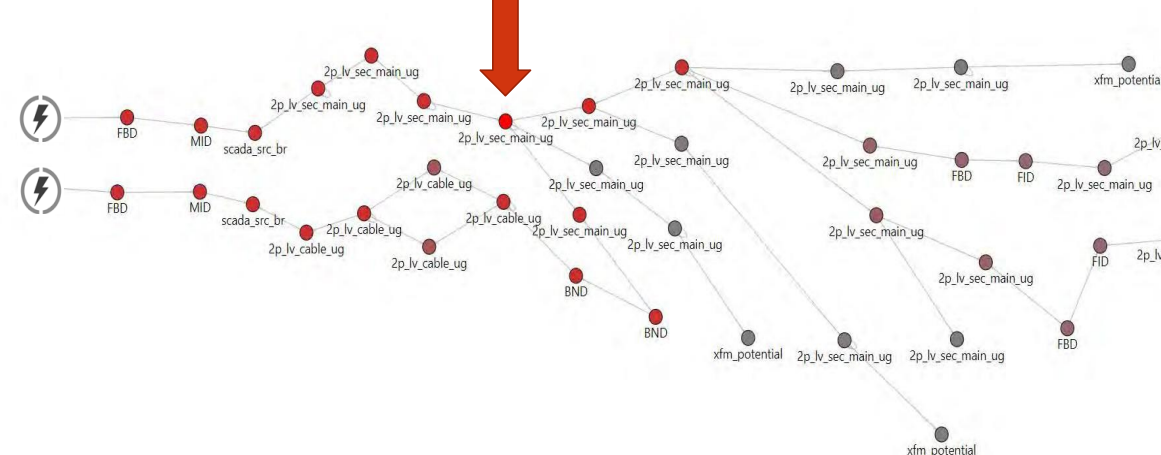
\includegraphics[scale=0.4]{Introduction/img/nodeimportant.png}
    \label{fig:nodeIMP}
\end{figure}
\\
Immaginiamo che questa sia una rete di trasporti. Il nodo puntato dalla freccia fa da raccordo tra le due linee. Se succede qualcosa in quel nodo, allora ne risente tutto il sistema. 
\newpage
\subsection{Introduzione alla Graph Analytics}

La \textbf{Graph Analytics}, o analisi dei grafi, è un insieme di tecniche e algoritmi utilizzati per studiare e analizzare strutture a grafo, con l'obiettivo di estrarre informazioni significative dalle relazioni tra entità.

I grafi sono una rappresentazione naturale per molti sistemi complessi del mondo reale: reti sociali, infrastrutture di trasporto, sistemi informatici, reti biologiche, strutture dati nei motori di ricerca, blockchain e molto altro. L’analisi di queste strutture può rivelare pattern, tendenze, anomalie e proprietà globali o locali del sistema.

\subsubsection*{Obiettivi dell'analisi dei grafi}

L'analisi dei grafi mira a rispondere a domande come:
\begin{itemize}
    \item Quali sono i nodi più importanti o influenti in una rete?
    \item Quali comunità o gruppi di nodi sono strettamente connessi tra loro?
    \item Esistono pattern o percorsi ricorrenti all'interno del grafo?
    \item Ci sono anomalie o comportamenti sospetti nella rete?
\end{itemize}

\subsubsection*{Tecniche comuni}

Tra le tecniche più comuni nella Graph Analytics troviamo:
\begin{itemize}
    \item \textbf{Centralità}: misura l'importanza relativa di un nodo (es. grado, betweenness, closeness, PageRank);
    \item \textbf{Community detection}: individua gruppi di nodi fortemente connessi (es. algoritmo di Louvain, modularità);
    \item \textbf{Shortest path}: calcola i percorsi minimi tra coppie di nodi (es. algoritmo di Dijkstra, Bellman-Ford);
    \item \textbf{Link prediction}: predice la probabilità che si formi un nuovo arco tra due nodi;
    \item \textbf{Anomaly detection}: rileva nodi o connessioni insolite rispetto alla struttura generale del grafo.
\end{itemize}

\subsubsection*{Applicazioni reali}

La Graph Analytics trova applicazione in numerosi settori:
\begin{itemize}
    \item \textbf{Social network}: analisi dell'influenza, identificazione di comunità, suggerimenti di amicizie;
    \item \textbf{Cybersecurity}: rilevamento di attacchi o intrusioni in una rete di computer;
    \item \textbf{Biologia computazionale}: studio delle interazioni tra proteine o geni;
    \item \textbf{E-commerce}: raccomandazioni di prodotti basate sulla rete di acquisti e preferenze;
    \item \textbf{Finanza}: rilevamento di frodi analizzando i flussi di denaro come un grafo.
\end{itemize}

\subsubsection*{Grafi matematici}

Il grafo è una coppia G = (V,E), dove V è una collezione di vertici V = $\{V_i, i=1,..,n\}$
e E una collezione di archi (edges) fatta in questo modo $E_{ij} = \{(V_i, V_j)\}$, $V_i \in V$, $V_j \in V$. Come disegnare un grafo: 
\\
\begin{figure}[th]
    \centering
    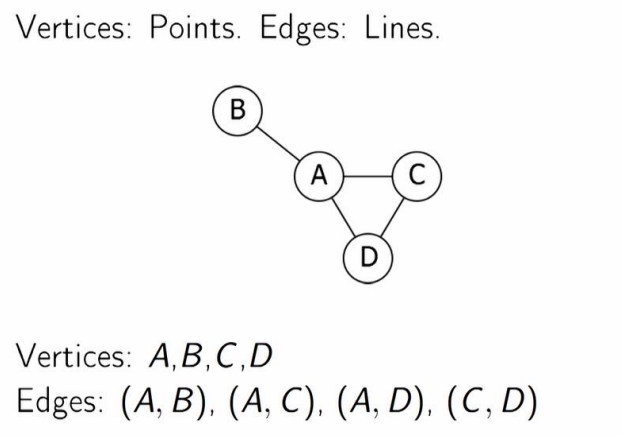
\includegraphics[scale=0.3]{Introduction/img/graphdesign.png}
    \label{fig:des}
\end{figure}

\subsubsection*{Vertici}

\textit{proprietà.} Un vertice può avere una label o essere unlabelled. Il numero dei vertici del grafo è anche detto \textbf{ordine del grafo}. 

\subsubsection*{Archi}

\textit{proprietà.} Un edge collega tra loro due vertici. I due vertici connessi prendono il nome di endpoints. Per definizione, se un edge esiste, allora esistono anche i suoi endpoints e sono 2. Se il grafo è diretto, allora esiste un outgoing edge (edge che esce) e un incoming edge (edge che entra).
\\
Il numero di edge stabilisce la \textbf{size} del grafo.
\newpage
\subsection{Il problema dei ponti di Königsberg}

Il problema dei \textbf{ponti di Königsberg} è considerato uno dei problemi fondamentali che ha dato origine alla \textbf{teoria dei grafi}. Esso fu affrontato e risolto da \textbf{Leonhard Euler} nel 1736.

\subsubsection*{Descrizione del problema}

La città di Königsberg (oggi Kaliningrad) era attraversata dal fiume Pregel, che formava due isole collegate tra loro e con le sponde del fiume tramite \textbf{sette ponti}. Il problema era il seguente:

\begin{quote}
    È possibile fare una passeggiata che attraversi ciascuno dei sette ponti \textbf{una sola volta} e che inizi e termini nello stesso punto?
\end{quote}

\subsubsection*{Modellazione tramite grafi}

Euler semplificò la situazione rappresentandola con un \textbf{grafo}:
\begin{itemize}
    \item Ogni \textbf{porzione di terra} (le due isole e le due sponde del fiume) viene rappresentata come un \textbf{nodo}.
    \item Ogni \textbf{ponte} viene rappresentato come un \textbf{arco} che collega due nodi.
\end{itemize}

In questo modo, il problema si traduce nel cercare un \textbf{ciclo euleriano}, ovvero un percorso chiuso che attraversi ogni arco del grafo \textbf{una sola volta}.

\subsubsection*{Soluzione di Euler}

Euler dimostrò che:
\begin{itemize}
    \item Un grafo possiede un \textbf{ciclo euleriano} se e solo se è connesso e \textbf{tutti i nodi hanno grado pari}.
    \item Un grafo possiede un \textbf{cammino euleriano} (che non torna al punto di partenza) se e solo se ha \textbf{esattamente due nodi di grado dispari}.
\end{itemize}

Nel caso del grafo dei ponti di Königsberg, \textbf{tutti e quattro i nodi} hanno un \textbf{numero dispari di archi} (cioè grado dispari), quindi:
\begin{itemize}
    \item \textbf{Non esiste} un ciclo euleriano;
    \item \textbf{Non esiste} nemmeno un cammino euleriano.
\end{itemize}

\subsubsection*{Conclusione}

Di conseguenza, non è possibile attraversare ciascun ponte una sola volta tornando al punto di partenza, né farlo iniziando e terminando in due punti diversi. Il problema dei ponti di Königsberg rappresenta quindi il primo esempio storico dell'applicazione della teoria dei grafi e ha segnato la nascita di questo importante campo della matematica.
\newpage
\begin{figure}[th]
    \centering
    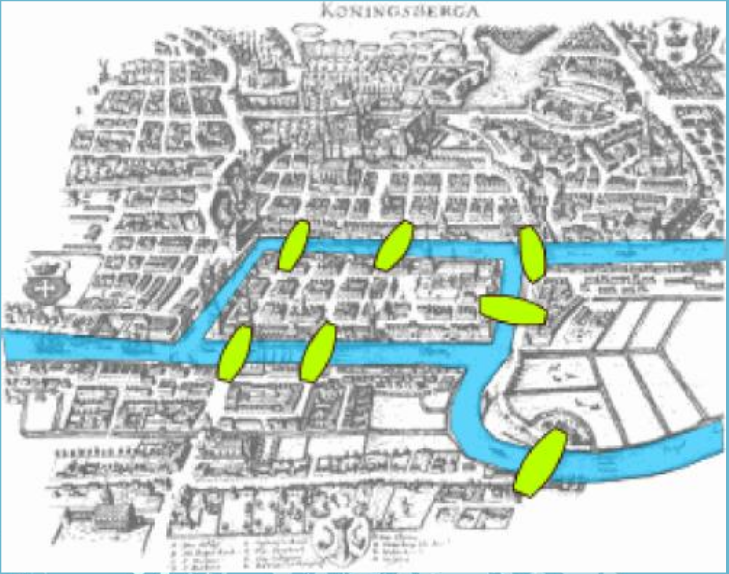
\includegraphics[scale=0.5]{Introduction/img/pontiKoningsberg.png}
    \caption{Immagine dei ponti di Koningsberg.}
\end{figure}
\newpage
\subsection{Proprietà dei grafi}

\subsubsection*{Grafi semplici e multigrafo}

Un grafo semplice (A) permette solo relazioni semplici, ovvero una singola interaction tra due nodi. Se dovessi avere la necessità di usare più relazioni tra due nodi allora si parla di multigrafo (B). 
\\
\begin{figure}[th]
    \centering
    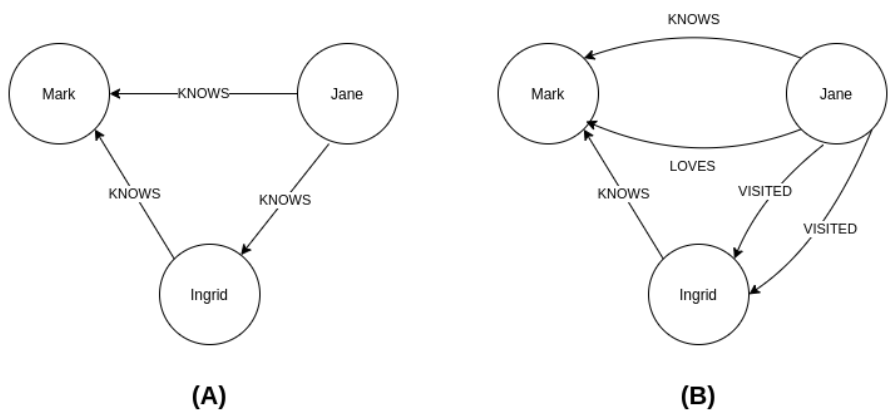
\includegraphics[scale=0.4]{Introduction/img/multigraph.png}
    \label{fig:multigraph}
\end{figure}

\subsubsection*{Grafi completi}

Due vertici si dicono \textbf{adiacenti} se sono connessi da un edge. Due edges invece si dicono \textbf{incidenti} se connettono lo stesso nodo ad altri nodi. 
\\
Posso quindi dire che se tutti vertici di un grafo sono a coppie adiacenti, il grafo è \textbf{}{completo}. In un grafo completo, tutti i nodi sono connessi tra loro. 
\\
\begin{figure}[th]
    \centering
    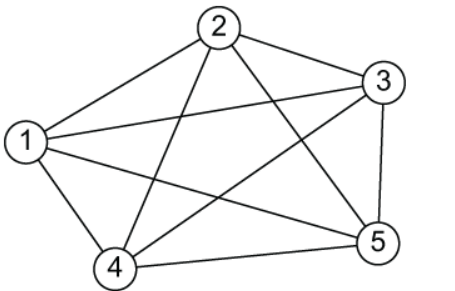
\includegraphics[scale=0.5]{Introduction/img/graphcomplete.png}
    \label{fig:complete}
\end{figure}

\subsubsection*{Indegree e Outdegree}

In un grafo diretto, il grado di un vertice V è diviso nell'\textbf{indegree} che consiste nel numero di edge per cui V è end node e \textbf{outdegree} che è il numero di edge per cui è start node.
\\
Una delle proprietà più importanti di un vertice è il suo grado: il numero di edge incidenti a tal vertice, che coincide anche con il numero dei nodi a lui adiacenti. 
\subsubsection*{Average degree}
Il grado medio è definito come segue:
\begin{center}
        \begin{math}
            a = \frac{1}{N} \sum_{i = 1,...,N} degree(V_i)
        \end{math}
\end{center}
Dove N è il numero di vertici nel grafo.

\subsubsection*{Percorsi}
 Una sequenza di vertici consecutivi connessi da degli edges si chiama \textbf{path} (percorso). Un path dove non ci sono vertici ripetuti è un \textbf{path semplice}. Un path dove il primo e l'ultimo vertice coincidono si chiama \textbf{cycle}. 
 \\
Un grafo che ha almeno un edge ha necessariamente un path. Se i vertici sono connessi con degli edge diretti (ovvero il grafo è diretto) possiamo chiamarlo \textbf{directed path}. Esistono diverse tipologie di grafi con diversi percorsi:
\begin{itemize}
    \item \textbf{weighted graphs:} sono dei grafi dove il passaggio da un vertice ad un altro ha un costo che è un valore numerico, che può essere utilizzato ad esempio in una rete di trasporti. 
    \item \textbf{monopartite graphs:} grafi dove tutti i nodi sono della stessa classe (es: persone, animali)
    \item \textbf{multipartite graphs:} grafi dove abbiamo più di una classe. Un grafo che ha esattamente due classi è chiamato bipartite graph.
\end{itemize}
\subsubsection*{La matrice di adiacenza}

Una delle modalità più comuni per rappresentare un grafo in forma computazionale è la \textbf{matrice di adiacenza}. Si tratta di una matrice quadrata che descrive la connessione tra i nodi del grafo.

\paragraph{Definizione}

Data un grafo $G = (V, E)$ con $n = |V|$ nodi, la sua \textbf{matrice di adiacenza} $A$ è una matrice $n \times n$ tale che:

\[
A_{ij} =
\begin{cases}
1 & \text{se esiste un arco da } v_i \text{ a } v_j, \\
0 & \text{altrimenti.}
\end{cases}
\]

Nel caso di grafi \textbf{non orientati}, la matrice di adiacenza è \textbf{simmetrica}, cioè $A_{ij} = A_{ji}$.

Nel caso di grafi \textbf{orientati}, la direzione degli archi è importante, quindi in generale $A_{ij} \neq A_{ji}$.

\paragraph{Esempio}

Consideriamo un grafo non orientato con tre nodi $V = \{v_1, v_2, v_3\}$ e archi $E = \{(v_1, v_2), (v_2, v_3)\}$. La sua matrice di adiacenza è:

\[
A =
\begin{bmatrix}
0 & 1 & 0 \\
1 & 0 & 1 \\
0 & 1 & 0
\end{bmatrix}
\]

\paragraph{Proprietà}

\begin{itemize}
    \item La riga $i$ della matrice rappresenta tutti i nodi a cui è connesso il nodo $v_i$.
    \item Il numero di $1$ nella riga (o colonna) $i$ corrisponde al \textbf{grado} del nodo $v_i$ (in grafi non orientati).
    \item Per grafi pesati, la matrice di adiacenza può contenere i \textbf{pesi} degli archi anziché solo $0$ e $1$.
\end{itemize}

\paragraph{Vantaggi e svantaggi}

\begin{itemize}
    \item \textbf{Vantaggi:} accesso immediato all'informazione su una connessione tra due nodi; utile per grafi densi.
    \item \textbf{Svantaggi:} utilizza molta memoria per grafi sparsi (\emph{sparse}), dove la maggior parte delle celle sono zeri.
\end{itemize}

\subsubsection*{Graph density}
La densità è un parametro che ci aiuta a stabilire quanto un grafo sia "pieno" tenendo conto del numero di edges che possiede e in relazione al numero dei suoi vertici. La densità di un grafo D ha questa forma D(V,E); questo valore oscilla tra 0 (grafo perfettamente sparse) e 1 (grafo completo, perfettamente denso). Per un grafo indiretto è:
\begin{center}
        \begin{math}
            D_U(V,E) = \frac{|E|}{Max_U(V)} = \frac{2 \times |E|}{|V| \times (|V| - 1)}
        \end{math}
\end{center}
Max(V) è il massimo numero di edges. E dipende dall'ordine ma non dalla size del grafo. E possiamo definire questo valore in relazione all'ordine: 
\begin{center}
        \begin{math}
            Max_U(V) = \frac{|V| (|V - 1|)}{2}
        \end{math}
\end{center}
La sua definizione possiamo estenderla ai grafi diretti:
\begin{center}
        \begin{math}
            Max_U(V) = |V| (|V - 1|) = 2 \times M_U(V)
        \end{math}
\end{center}
Se il grafo è diretto, il numero massimo di edges è il doppio del caso non diretto. Di conseguenza la densità nel caso diretto sarà la metà del caso non diretto. 
\paragraph*{Sparse vs Dense}
Un grafo sparse è un grafo dove la densità D è nel range più basso possibile di codominio (D compreso tra 0 e $\frac{1}{2}$). Analogamente, un grafo denso ha un range del codominio più ampio (D compreso tra $\frac{1}{2}$ e 1). Se D = $\frac{1}{2}$ non viene considerato da nessuno dei due tipi.  
\paragraph*{Condizioni generali}
\begin{itemize}
    \item la densità di un grafo di ordine 1 è indefinita, per ovvie ragioni
    \item tutti i grafi vuoti hanno densità 0
    \item tutti i grafi completi anno densità 1
    \item un grafo non diretto ha una densità di almeno $\frac{2}{|V|}$ quindi è garantito che sia denso per $ |V| < 4$
    \item un grafo diretto tracciabile non è sempre detto che sia denso
\end{itemize}
\paragraph*{Efficiency in Graph Storage}
La densità di un grafo influisce sull'efficienza dello storage del grafo in memoria. I grafi sono strutture molto complesse e devono essere salvate in maniera efficiente. Esistono quindi due tipi di rappresentazioni. lista di edges, o adjacency matrix. Come regola generale, se il grafo è sparso, usa lista di edges, altrimenti usa la adjacency matrix (per i più densi). 
\paragraph*{Walk, Trail e Path}
\begin{itemize}
    \item walk: un walk è un cammino generico che possiamo percorrere nel nostro grafo. 
    \item trail: un trail è un walk che non ripassa per lo stesso edge più di una volta. Se è un percorso chiuso, prende il nome di circuit.
    \item path: un path è un walk che non ripassa due volte per lo stesso vertice.
\end{itemize}

\subsection*{Grafi euleriani, non euleriani e semi-euleriani}

Nella teoria dei grafi, un problema classico consiste nel determinare se esiste un percorso che attraversi ogni arco del grafo una sola volta. Questo porta alla definizione di grafi \textbf{euleriani}, \textbf{semi-euleriani} e \textbf{non euleriani}, concetti introdotti da Leonhard Euler.

\subsubsection*{Grafo euleriano}

Un \textbf{grafo euleriano} è un grafo in cui esiste un \textbf{ciclo euleriano}, cioè un ciclo che:
\begin{itemize}
    \item attraversa \textbf{ogni arco esattamente una volta};
    \item \textbf{inizia e termina nello stesso nodo}.
\end{itemize}

\paragraph{Condizione necessaria e sufficiente (non orientato):}
Un grafo non orientato è euleriano se e solo se:
\begin{itemize}
    \item il grafo è \textbf{connesso} (eccetto i nodi isolati);
    \item \textbf{tutti i nodi hanno grado pari}.
\end{itemize}

\paragraph{Esempio:} Un ciclo chiuso in cui ogni nodo ha due archi è un grafo euleriano.

\subsubsection*{Grafo semi-euleriano}

Un \textbf{grafo semi-euleriano} è un grafo in cui esiste un \textbf{cammino euleriano}, cioè un percorso che:
\begin{itemize}
    \item attraversa \textbf{ogni arco esattamente una volta};
    \item \textbf{inizia e termina in nodi diversi}.
\end{itemize}

\paragraph{Condizione necessaria e sufficiente (non orientato):}
Un grafo è semi-euleriano se e solo se:
\begin{itemize}
    \item è connesso;
    \item \textbf{esattamente due nodi hanno grado dispari}.
\end{itemize}

\paragraph{Esempio:} Un grafo a forma di catena con due estremi di grado dispari è semi-euleriano.

\subsubsection*{Grafo non euleriano}

Un \textbf{grafo non euleriano} è un grafo che \textbf{non possiede né un ciclo euleriano né un cammino euleriano}. Questo accade quando:
\begin{itemize}
    \item il grafo non è connesso (escludendo nodi isolati), oppure
    \item contiene \textbf{più di due nodi con grado dispari}.
\end{itemize}

\paragraph{Esempio:} Il grafo dei \emph{ponti di Königsberg} è un classico esempio di grafo non euleriano: ha quattro nodi con grado dispari, quindi non è possibile attraversare ogni ponte una sola volta, né con partenza e arrivo nello stesso punto, né in punti diversi.

\subsubsection*{Nota sui grafi orientati}

Nei grafi \textbf{orientati}, le condizioni per l'esistenza di un cammino o ciclo euleriano sono leggermente diverse e si basano su:
\begin{itemize}
    \item \textbf{Grado entrante} (\emph{in-degree}) e \textbf{grado uscente} (\emph{out-degree}) dei nodi;
    \item \textbf{Forte connessione} del grafo.
\end{itemize}

\begin{itemize}
    \item Un grafo orientato ha un ciclo euleriano se è fortemente connesso e ogni nodo ha in-degree uguale a out-degree.
    \item Ha un cammino euleriano (semi-euleriano) se è connesso e:
    \begin{itemize}
        \item Un nodo ha out-degree = in-degree + 1 (inizio del cammino),
        \item Un nodo ha in-degree = out-degree + 1 (fine del cammino),
        \item Tutti gli altri nodi hanno in-degree = out-degree.
    \end{itemize}
\end{itemize}
\newpage
\section{Algoritmi di ricerca nei grafi}
\subsection*{DFS e BFS}
\subsubsection*{Depth First Search (DFS)}

Il \textit{Depth First Search} (DFS) è un algoritmo di visita dei grafi che esplora il grafo andando il più in profondità possibile lungo ciascun ramo prima di fare \textit{backtracking}.

\begin{itemize}
    \item Funziona sia su grafi orientati che non orientati.
    \item Può essere implementato in modo ricorsivo o iterativo (usando uno \texttt{stack}).
    \item È utile per:
    \begin{itemize}
        \item Rilevare cicli
        \item Trovare componenti connesse
        \item Ordinamento topologico (nei grafi aciclici orientati)
    \end{itemize}
\end{itemize}

\paragraph{Algoritmo (versione ricorsiva):}

\begin{verbatim}
DFS(G, u):
    visited[u] = true
    for each v in adjacency_list[u]:
        if not visited[v]:
            DFS(G, v)
\end{verbatim}

\paragraph{Complessità:}
\begin{itemize}
    \item Tempo: $\mathcal{O}(V + E)$
    \item Spazio: $\mathcal{O}(V)$ per la memoria usata dai nodi visitati (più lo stack della ricorsione)
\end{itemize}

\subsubsection*{Breadth First Search (BFS)}

Il \textit{Breadth First Search} (BFS) è un algoritmo di visita dei grafi che esplora tutti i nodi vicini prima di procedere a quelli più lontani. Utilizza una \texttt{queue} (coda FIFO).

\begin{itemize}
    \item Visita i nodi per livelli (distanza minima in termini di archi dal nodo sorgente).
    \item Può essere usato per:
    \begin{itemize}
        \item Trovare il cammino minimo in grafi non pesati
        \item Rilevare componenti connesse
    \end{itemize}
\end{itemize}

\paragraph{Algoritmo:}

\begin{verbatim}
BFS(G, s):
    queue = [s]
    visited[s] = true
    while queue is not empty:
        u = queue.pop()
        for each v in adjacency_list[u]:
            if not visited[v]:
                visited[v] = true
                queue.append(v)
\end{verbatim}

\paragraph{Complessità:}
\begin{itemize}
    \item Tempo: $\mathcal{O}(V + E)$
    \item Spazio: $\mathcal{O}(V)$ per la memoria dei nodi visitati e la coda
\end{itemize}


\subsection*{Shortest Path}
Il concetto più importante nella scelta di un path è sicuramente la scelta del path più veloce, più comodo, di fatto più corto. Questo prenderà il nome di \textbf{shortest path}. Esso cambia in base al tipo di grafo:
\begin{itemize}
    \item se il grafo non è pesato, basta trovare il numero minore di edges da percorrere.
    \item se il grafo è pesato, basta trovare il percorso (path) con il peso totale minore. 
\end{itemize}
Ma quali sono i possibili percorsi? Dipende dalla richiesta:
\begin{itemize}
    \item parto da un solo Vertice (nodo) $\rightarrow$ dato un nodo di partenza trova il percorso più veloce per connetterlo a tutti gli altri. 
    \item data una partenza, trova la strada più veloce per la destinazione. Fondamentalmente è il discorso che fa Google Maps. \textbf{Se esiste il percorso}. 
    \item trova tutti gli shortest path che collegano tra loro tutti i diversi nodi del grafo. 
\end{itemize}
Il BFS come metodo di ricerca, è sicuramente il più complesso.
\newpage
\subsubsection*{Applicazioni}
Sicuramente la ricerca del cammino più breve trova facile impiego nel campo della ricerca stradale. Infatti, è semplice pensare di attribuire ad ogni incrocio un nodo e le strade sono gli edges, come in figura qui sotto: 
\\
\begin{figure}[th]
    \centering
    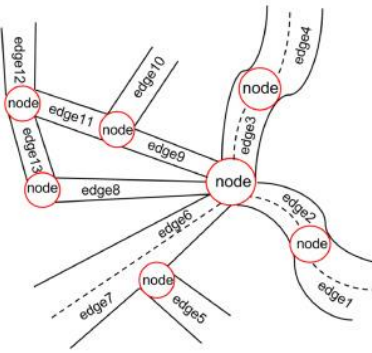
\includegraphics[scale=0.4]{Introduction/img/roadmap.png}
    \label{fig:roadmap}
\end{figure}
\\[3ex]
Potrebbe essere anche utile attribuire ad ogni edge un peso che può significare il tempo di percorrenza della strada, la lunghezza, ecc... Usare edge diretti può essere utile per rappresentare le strade a senso unico. Esiste un algoritmo chiamato Hub Labeling capace di calcolare lo shortest path di tutte le strade in EU o in USA in frazioni di secondo. 
\subsection{Connettività di un grafo}
La connettività in un grafo è la qualità delle connessioni tra i suoi vertici. Si fa distinzione tra grafo connesso e disconnesso: 
\\
\begin{figure}[th]
    \centering
    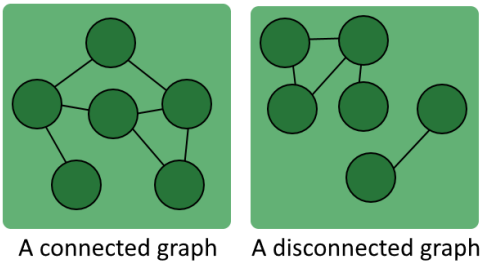
\includegraphics[scale=0.4]{Introduction/img/grafoconnessodisconnesso.png}
    \label{fig:connessodisc}
\end{figure}
\subsubsection*{Max-Flow Min-Cut Theorem}

Sia \( G = (V, E) \) un grafo orientato con:
\begin{itemize}
    \item una sorgente \( s \in V \),
    \item un pozzo (sink) \( t \in V \),
    \item una funzione di capacità \( c: E \rightarrow \mathbb{R}^+ \).
\end{itemize}

Un \textbf{flusso} \( f: E \rightarrow \mathbb{R} \) deve rispettare:
\begin{enumerate}
    \item \textbf{Vincolo di capacità:} \( 0 \leq f(u,v) \leq c(u,v) \)
    \item \textbf{Conservazione del flusso:} per ogni nodo \( v \neq s, t \),
    \[
    \sum_{u \in V} f(u,v) = \sum_{w \in V} f(v,w)
    \]
\end{enumerate}

Il \textbf{valore del flusso} è definito come:
\[
|f| = \sum_{v \in V} f(s,v)
\]

\paragraph{Taglio \( (S, T) \):} una partizione dei nodi \( V \) tale che \( s \in S \), \( t \in T \), e \( S \cup T = V \), \( S \cap T = \emptyset \).

La \textbf{capacità del taglio} è:
\[
c(S, T) = \sum_{\substack{u \in S, v \in T \\ (u,v) \in E}} c(u,v)
\]

\paragraph{Teorema:} Il massimo flusso da \( s \) a \( t \) è uguale alla capacità minima di un taglio che separa \( s \) da \( t \):
\[
\max_f |f| = \min_{(S,T)} c(S,T)
\]

\subparagraph{Conseguenze:}
\begin{itemize}
    \item Ogni flusso massimo attraversa un taglio minimo.
    \item Il taglio minimo fornisce un limite superiore al flusso.
    \item Quando l’algoritmo trova un flusso massimo, ha anche trovato un taglio minimo.
\end{itemize}

Parlando per un grafo, questo significa cercare il minimo numero di edges che se rimossi, rendono il grafo disconnesso. Il flusso inteso qui può essere qualunque cosa, ad esempio anche un flusso di dati che passa attraverso un computer network come internet. 

\subsubsection*{Eccentricity}
L'eccentricity di un nodo è la distanza massima da percorrere per raggiungere il nodo \textbf{più lontano} partendo da quello attuale. Tramite questa grandezza è possibile definire: 
\begin{itemize}
    \item raggio di un grafo: l'eccentricità minima di ogni nodo nel grafo. 
    \item diametro di un grafo: la massima eccentricità di ogni nodo nel grafo. 
\end{itemize}
\subsubsection*{Connected components}
Il component di un grafo sono tutte le partizioni separate dal grafo completo. Ovvero tutte le parti del grafo a sè stanti. Se un grafo ha un unica componente, si dice che è un grafo \textbf{CONNESSO} altrimenti si dirà \textbf{DISCONNESSO} e si conteranno le partizioni chiamandole componenti. 
\newpage
\subsubsection*{Disconnected w/ 2 components}
\begin{figure}[th]
    \centering
    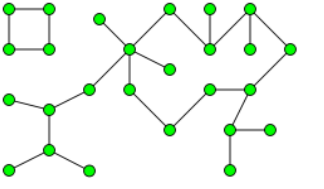
\includegraphics[scale=0.4]{Introduction/img/disconnected.png}
    \label{fig:disconnected}
\end{figure}
\subsubsection*{Connected w/ 1 component}
\begin{figure}[th]
    \centering
    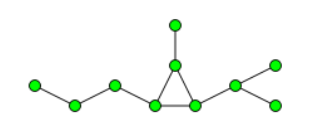
\includegraphics[scale=0.4]{Introduction/img/connected.png}
    \label{fig:connected}
\end{figure}

\subsubsection*{Strongly connected components}
Uno \textbf{strongly connected component} è una porzione di un grafo diretto dove c'è un path diretto tra tutti i nodi. 
\\
\begin{figure}[th]
    \centering
    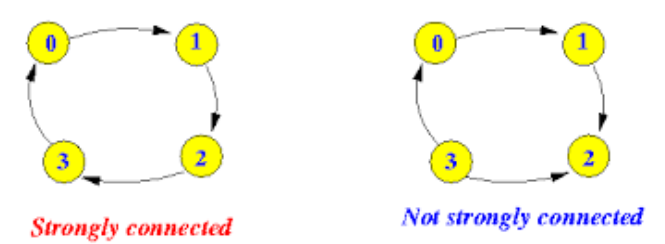
\includegraphics[scale=0.4]{Introduction/img/stronglyconnected.png}
    \label{fig:stronglyconnected}
\end{figure}

\subsubsection*{Conduttanza nei Grafi}

La \textbf{conduttanza} (\textit{conductance}) è una misura che quantifica quanto bene un sottografo è separato dal resto del grafo. È molto usata nell'analisi di reti e nel clustering di grafi.

\paragraph{Definizione:}

Dato un grafo non orientato \( G = (V, E) \), e un sottoinsieme non vuoto di nodi \( S \subset V \), la conduttanza di \( S \) è definita come:

\[
\phi(S) = \frac{|\partial S|}{\min(\mathrm{vol}(S), \mathrm{vol}(V \setminus S))}
\]

dove:
\begin{itemize}
    \item \( \partial S \) è l'insieme degli archi che collegano un nodo in \( S \) a un nodo in \( V \setminus S \) (il bordo del taglio),
    \item \( |\partial S| \) è il numero di tali archi,
    \item \( \mathrm{vol}(S) = \sum_{v \in S} \deg(v) \) è il volume di \( S \), cioè la somma dei gradi dei nodi in \( S \).
\end{itemize}
In un grafo non orientato bisogna considerare entrambe le direzioni di un edge. 
\paragraph{Interpretazione:}
\begin{itemize}
    \item Una bassa conduttanza \( \phi(S) \) indica che il sottoinsieme \( S \) è \textit{ben separato} dal resto del grafo: pochi archi lo collegano al resto rispetto alla sua dimensione.
    \item Un valore elevato di \( \phi(S) \) indica invece che \( S \) è \textit{fortemente connesso} al resto del grafo.
\end{itemize}

\paragraph{Conduttanza del grafo:}

La conduttanza del grafo è definita come la conduttanza del taglio migliore:

\[
\phi(G) = \min_{\substack{S \subset V \\ 0 < \mathrm{vol}(S) \leq \mathrm{vol}(V)/2}} \phi(S)
\]
Banalmente, data la partizione di un grafo in due set disgiunti G1 e G2, la conduttanza consiste nella somma degli edges che vanno da G1 a G2 diviso il minimo tra gli edges che vanno da G1 a G2. 
\paragraph{Applicazioni:}
\begin{itemize}
    \item Clustering e rilevamento di comunità in grafi
    \item Algoritmi di partizionamento dei grafi
    \item Analisi della connettività di reti complesse
\end{itemize}

\subsubsection*{Clique nei Grafi}

Sia \( G = (V, E) \) un grafo non orientato.

Un \textbf{clique} è un sottoinsieme di vertici \( C \subseteq V \) tale che ogni coppia distinta di vertici in \( C \) è connessa da un arco in \( E \), ovvero:

\[
\forall u, v \in C, \quad u \neq v \Rightarrow (u,v) \in E
\]

\paragraph{Tipi di clique:}
\begin{itemize}
    \item \textbf{Clique massimale:} un clique che non può essere esteso includendo un altro nodo adiacente (cioè non è contenuto in nessun altro clique più grande).
    \item \textbf{Clique massimo:} un clique con il massimo numero possibile di nodi nel grafo.
    \item \textbf{k-clique:} un clique composto da esattamente \( k \) nodi.
\end{itemize}

\paragraph{Esempio:}
Nel grafo seguente (non rappresentato), se i nodi \( \{1, 2, 3\} \) sono tutti connessi tra loro, allora formano un 3-clique.

\paragraph{Applicazioni:}
\begin{itemize}
    \item Analisi di reti sociali (gruppi di amici tutti connessi tra loro)
    \item Bioinformatica (moduli funzionali nelle reti genetiche)
    \item Ottimizzazione e intelligenza artificiale
\end{itemize}

\paragraph{Complessità computazionale:}
Il problema di trovare un clique massimo è \textbf{NP-completo}. Trovare tutti i cliques massimali è computazionalmente costoso per grafi grandi, ma esistono algoritmi efficienti per casi particolari (es. algoritmo di Bron–Kerbosch). [Fonte GPT]

\subsubsection*{K-Core Decomposition}
Graph algorithm che serve per cercare il piú grande sottografo dove tutti i nodi hanno almeno grado k. Il sottografo massimo prende il nome di \textbf{k-core} del grafo. 
\\
L'algoritmo iterativamente rimuove i nodi con un grado minore di k e tutti i nodi incidenti ad essi finché non rimangono solo nodi con degree almeno uguale a k. 

\subsection{Graph Structure Analysis}
Nell'analisi delle strutture dei grafi, é utile evidenziare due componenti principali:
\begin{itemize}
    \item \textbf{Average Diameter L}: misura media dello shortest path che collega tra loro due nodi qualsiasi.
    \\
    Misura quanto i nodi siano "lontani" tra loro. 
    \[
    L =\frac{1}{N(N-1)} \sum_{i \neq j} d(i,j)
    \]
    Dove N é il numero di nodes e d(i,j) shortest path tra il nodo i e j.
    \item \textbf{Clustering Coefficient C}: media della local density.
    É equivalente alla densitá del sottografo quando si considerano solo i vicini di n, escludendo n. Questo misura quanto i suoi vicini siano tendenti ad essere un clique (sottografo completo) e quindi misura quanto due nodi vicini al nodo target possano essere connessi.
    \\[2ex]
    \textbf{Directed:}\[
    C_n = \frac{|E|}{|V|(|V|-1)}
    \]
    \\
    \textbf{Undirected:}\[
    C_n = \frac{2|E|}{|V|(|V|-1)}
    \]    
    \\
    \textbf{Clustering Coefficient of the entire graph:}
    \[
    C = \frac{1}{|N|}\sum_{n \in N}C_n
    \]
\end{itemize}

\subsubsection*{Wiener Index: closeness of a graph}
Il wiener index é una misura della complessitá topologica definita come la somma a coppie degli shortest paths tra i nodi del grafo. 
\newpage
\subsection{Centrality of a node}
É la misura dell'importanza di un nodo all'interno di un grafo. La banale intuizione é che piú un nodo é fondamentale nel mantenere un grafo connesso, piú il nodo é importante. 
\\
Vengono utilizzate diverse metriche per indicare la \textbf{centrality} di un nodo:
\begin{itemize}
    \item \textbf{Degree centrality}: numero dei vicini del nodo v 
    \item \textbf{Closeness centrality}: reciproco della distanza tra un nodo qualsiasi v e tutti gli altri nodi:
    \[
    C_c (v)=\frac{1}{\sum_{u \in V} \delta (u,v)}
    \]
    Dove il termine in delta é la distanza tra il nodo u e v.
    \item \textbf{Betweenness centrality [0-1]}: rapporto tra il numero di shortest paths passanti per il nodo v e tutti gli shortest paths del grafo:
    \[
    C_B(v)=\sum_{s\neq t \neq v \in V} \frac{\sigma_{st}(v)}{\sigma_{st}}
    \]
    Dove sigma indica il numero di shortest paths (in particolare quello di v indica quelli passanti per v)
\end{itemize}
\paragraph{Esempio.}
Il nodo di cui valutare l'importanza é $n$. 
\begin{figure}[th]
    \centering
    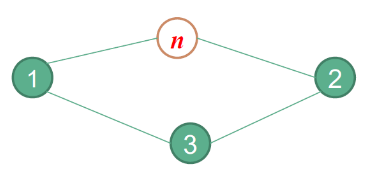
\includegraphics[scale=0.5]{Introduction//img/image.png}
\end{figure}
Grafo indiretto, 4 nodi totali. I parametri:
\begin{itemize}
    \item \textbf{Degree centrality}=2 
    \item \textbf{Closeness $C_C(n)$}= $\frac{1}{1+1+2}$ distanza di $n$ dagli altri nodi. Risultato: $0.25$
    \item \textbf{Betweenness $C_B$}: Per questo punto, é necessario scrivere tutti gli shortest paths:
    \begin{table}[th]
        \centering
        \begin{tabular}{c|c}
            CASO & Shortest Path \\
            P[1,n] & (1, n) \\
            P[2, n] & (2, n) \\
            P[3, 1] & (3, 1) \\
            P[3, 2] & (3, 2) \\
            P[1, 2] & (1, 3, 2), (1, n, 2) \\
            P[3, n] & (3, 2, n), (3, 1, n) \\
        \end{tabular}
    \end{table}
    Casi totali: 8. Quanti contengono $n$? 5. Quindi il ratio risulta $\frac{5}{8}$. 
\end{itemize}

\subsection{Centrality Measures}
Il concetto di "importanza" all'interno di una rete può essere interpretato in molti modi diversi, e per questo esistono varie misure di centralità che permettono di quantificare tale importanza in base alla struttura del grafo e al ruolo che ogni nodo ricopre nel contesto della rete. Tra le più comuni troviamo:

\begin{itemize}
  \item \textbf{PageRank}: Questa misura di centralità è stata originariamente sviluppata da Google per classificare le pagine web. L'algoritmo assegna un punteggio a ciascun nodo del grafo basandosi sia sul numero di archi (link o connessioni) che entrano nel nodo, sia sulla qualità dei nodi da cui provengono tali connessioni. In sostanza, un nodo riceve un punteggio elevato se è collegato da altri nodi che sono anch'essi importanti. Questo tipo di centralità è particolarmente utile in contesti in cui la popolarità o l’autorevolezza gioca un ruolo fondamentale.

  \item \textbf{Centralità di intermediazione (Betweenness Centrality)}: Questo tipo di misura valuta quanto un nodo sia "strategico" nella rete, ovvero quanto spesso si trova sui cammini minimi (shortest paths) tra coppie di altri nodi. Un nodo con alta centralità di intermediazione agisce come ponte tra diverse parti del grafo e può quindi avere un ruolo critico nel facilitare (o controllare) il flusso di informazioni. È utile per individuare nodi influenti nel collegare comunità o sottoreti diverse.
\end{itemize}

Queste misure sono fondamentali in numerose applicazioni di analisi dei grafi, come la rilevazione di influencer nei social network, l’identificazione di nodi critici in reti infrastrutturali, la valutazione dell’impatto di un'entità all’interno di un ecosistema complesso o l’ottimizzazione della diffusione di informazioni.

\paragraph{TextRank} L'algoritmo TextRank, introdotto da Mihalcea e Tarau nel 2004, è un metodo di classificazione basato su grafi utilizzato per l'elaborazione del linguaggio naturale, in particolare per compiti come l'estrazione automatica di parole chiave e la sintesi automatica. L'applicazione dell'algoritmo su testi scritti prevede i seguenti passaggi:

\begin{enumerate}
  \item \textbf{Identificazione delle unità testuali rilevanti}: Vengono individuate le unità testuali pertinenti al compito specifico (ad esempio, parole o frasi significative) e aggiunte al grafo come nodi.

  \item \textbf{Identificazione delle relazioni tra le unità testuali}: Si determinano le relazioni che collegano le unità testuali. Gli archi del grafo possono essere diretti o non diretti, e pesati o non pesati, a seconda del tipo di relazione e della sua intensità.

  \item \textbf{Esecuzione iterativa dell'algoritmo di ranking}: L'algoritmo di ordinamento basato su grafo viene applicato in modo iterativo fino al raggiungimento della convergenza (ovvero, quando i punteggi dei nodi si stabilizzano) oppure fino al raggiungimento del numero massimo di iterazioni.

  \item \textbf{Ordinamento e selezione}: I nodi vengono ordinati in base ai punteggi finali ottenuti, e tali punteggi vengono utilizzati per effettuare decisioni di ordinamento o selezione. A questo punto è possibile anche unire due o più unità testuali in un’unica parola chiave o frase chiave.
\end{enumerate}

Questo approccio consente di estrarre in modo efficace informazioni rilevanti da un testo, sfruttando la struttura delle relazioni tra le parole piuttosto che un'analisi puramente statistica.

\newpage

\subsection{Community Detection}
Una community all'interno di un grafo corrisponde ad una porzione interna con un'alta connetivitá spesso chiamata anche \textbf{cluster}. Questi gruppi si riconoscono perché hanno una bassa connetivitá con gli altri nodi del grafo, ma un'alta connetivitá tra loro. 
\\
Per fare community detection ovvero trovare le community all'interno di un grafo, é necessario utilizzare l'algoritmo di \textbf{Girvan-Newman}: 
\begin{enumerate}
    \item \textbf{Calcolare l'edge betweenness:} trova gli edge piú centrali all'interno del grafo.
    \item \textbf{Elimina}: elimina gli edges con alta betweenness.
    \item \textbf{Trova}: tutti i componenti connessi rimanenti sono comminities. Processo che puó essere iterato. 
\end{enumerate}
Vengono cercati gli edges piú importanti, e vengono prunati. In questo modo, avanzano quelli un po' meno rilevanti, non abbastanza da diventare i piú centrali. Ma quelli che comunque hanno tante connessioni: quindi sono edge che connettono tanti nodi insieme in quelle che chiamiamo communities. 

\subsection{Graph Partitioning}
Nei paragrafi precedenti é stato introdotto il concetto di "dividere" il grafo in piú parti, tagliando degli archi. 
\paragraph{Definizione} L'idea é quella di mantenere le parti in cui dividiamo densamente connesse e di usare il minor numero di tagli possibile. \textbf{Graph Cut} é proprio ricercare di avere dei grafi distinti dopo il taglio. Il nostro cut quindi dovrá minimizzare la conduttanza: 
\[
C(G_1, G_2) = \frac{|\mathbb{C}|}{min\{\mathbb{C} + |G_1|), (\mathbb{C} + G_2)\}}
\]
Dove $\mathbb{C}$ é il Cut:
\[
|Cut(G_1, G_2)|
\]

\subsubsection*{Proximity Prestige nei Grafi}

Il \textbf{Proximity Prestige} è una misura di centralità usata per valutare il prestigio di un nodo all'interno di un grafo diretto, tenendo conto sia della quantità di nodi che possono raggiungerlo, sia della distanza con cui lo fanno. È un'estensione del concetto di \textit{prestige} (cioè di essere destinatario di connessioni), che integra l’idea di \textit{prossimità}.

\paragraph{Definizione}

Dato un grafo diretto \( G = (V, E) \), il \textbf{Proximity Prestige} di un nodo \( v \in V \) si definisce come:

\[
\text{ProxPrestige}(v) = \frac{|\text{R}(v)|}{n-1} \cdot \frac{1}{\frac{1}{|\text{R}(v)|} \sum_{u \in \text{R}(v)} d(u, v)}
\]

dove:
\begin{itemize}
    \item \( \text{R}(v) \) è l'insieme dei nodi che possono raggiungere \( v \) tramite un cammino diretto (cioè i predecessori di \( v \)) anche chiamato \textbf{Influence Domain}, 
    \item \( d(u, v) \) è la lunghezza del cammino più breve da \( u \) a \( v \),
    \item \( n \) è il numero totale di nodi nel grafo.
\end{itemize}

La formula può essere letta come:

\[
\text{ProxPrestige}(v) = \text{Coverage}(v) \cdot \frac{1}{\text{Average Distance to } v}
\]

\paragraph{Interpretazione}

\begin{itemize}
    \item Il primo termine (\( \frac{|\text{R}(v)|}{n-1} \)) misura la \textit{copertura}, ossia la percentuale di nodi che possono raggiungere \( v \).
    \item Il secondo termine valuta l'\textit{efficienza con cui} tali nodi raggiungono \( v \), ovvero quanto in media sono vicini.
\end{itemize}

Un nodo ha \textbf{alto proximity prestige} se è raggiunto da molti altri nodi e questi lo raggiungono con cammini brevi.

\paragraph{Applicazioni}

Questa misura è utile in reti sociali, reti di citazioni e sistemi di comunicazione, per identificare gli attori più influenti non solo in base alla quantità di connessioni in entrata, ma anche alla rapidità con cui l’informazione può arrivare a loro.

